\documentclass[11pt, % The default document font size, options: 10pt, 11pt, 12pt
codirector, % Uncomment to add a codirector to the title page
]{charter} 




% El títulos de la memoria, se usa en la carátula y se puede usar el cualquier lugar del documento con el comando \ttitle
\titulo{Telemetría y posicionamiento de antena para interferometría} 

% Nombre del posgrado, se usa en la carátula y se puede usar el cualquier lugar del documento con el comando \degreename
\posgrado{Carrera de Especialización en Sistemas Embebidos} 
%\posgrado{Carrera de Especialización en Internet de las Cosas} 
%\posgrado{Carrera de Especialización en Intelegencia Artificial}
%\posgrado{Maestría en Sistemas Embebidos} 
%\posgrado{Maestría en Internet de las cosas}

% Tu nombre, se puede usar el cualquier lugar del documento con el comando \authorname
\autor{Valdez Gastón } 

% El nombre del director y co-director, se puede usar el cualquier lugar del documento con el comando \supname y \cosupname y \pertesupname y \pertecosupname
\director{Elias Fliger}
\pertenenciaDirector{IAR} 
% FIXME:NO IMPLEMENTADO EL CODIRECTOR ni su pertenencia
\codirector{Guillermo Gancio} % para que aparezca en la portada se debe descomentar la opción codirector en el documentclass
\pertenenciaCoDirector{IAR}

% Nombre del cliente, quien va a aprobar los resultados del proyecto, se puede usar con el comando \clientename y \empclientename
\cliente{Responsable del área de electrónica}
\empresaCliente{Instituto Argentino de Radioastronomía}

% Nombre y pertenencia de los jurados, se pueden usar el cualquier lugar del documento con el comando \jurunoname, \jurdosname y \jurtresname y \perteunoname, \pertedosname y \pertetresname.
\juradoUno{Nombre y Apellido (1)}
\pertenenciaJurUno{pertenencia (1)} 
\juradoDos{Nombre y Apellido (2)}
\pertenenciaJurDos{pertenencia (2)}
\juradoTres{Nombre y Apellido (3)}
\pertenenciaJurTres{pertenencia (3)}
 
\fechaINICIO{30 de abril de 2022}		%Fecha de inicio de la cursada de GdP \fechaInicioName
\fechaFINALPlan{18 de junio de 2021} 	%Fecha de final de cursada de GdP
\fechaFINALTrabajo{15 de mayo de 2022}	%Fecha de defensa pública del trabajo final

 \setlength{\parindent}{6pt} 			%sangria ! 
\begin{document}

\maketitle
\thispagestyle{empty}
\pagebreak


\thispagestyle{empty}
{\setlength{\parskip}{0pt}
\tableofcontents{}
}
\pagebreak


\section*{Registros de cambios}
\label{sec:registro}


\begin{table}[ht]
\label{tab:registro}
\centering
\begin{tabularx}{\linewidth}{@{}|c|X|c|@{}}
\hline
\rowcolor[HTML]{C0C0C0} 
Revisión & \multicolumn{1}{c|}{\cellcolor[HTML]{C0C0C0}Detalles de los cambios realizados} & Fecha      \\ \hline
0      & Creación del documento                                 &\fechaInicioName \\ \hline
%1      & Se completa hasta el punto 4 inclusive                 & dd/mm/aaaa \\ \hline
%2      & Se completa hasta el punto 7 inclusive
%		  Se puede agregar algo más \newline
%		  En distintas líneas \newline
%		  Así                                                    & dd/mm/aaaa \\ \hline
%3      & Se completa hasta el punto 11 inclusive                & dd/mm/aaaa \\ \hline
%4      & Se completa el plan	                                 & dd/mm/aaaa \\ \hline
\end{tabularx}
\end{table}

\pagebreak



\section*{Acta de constitución del proyecto}
\label{sec:acta}

\begin{flushright}
Buenos Aires, \fechaInicioName
\end{flushright}

\vspace{2cm}

Por medio de la presente se acuerda con el Ing. \authorname que su Trabajo Final de la \degreename se titulará ``\ttitle'', consistirá en la implementación de un sistema de posicionamiento y telemetría de una antena de plato parabólico y tendrá un presupuesto preliminar estimado de 800 hs de trabajo, con fecha de inicio \fechaInicioName y fecha de presentación pública \fechaFinalName.

Se adjunta a esta acta la planificación inicial.

\vfill

% Esta parte se construye sola con la información que hayan cargado en el preámbulo del documento y no debe modificarla
\begin{table}[ht]
\centering
\begin{tabular}{ccc}
\begin{tabular}[c]{@{}c@{}}Ariel Lutenberg \\ Director posgrado FIUBA\end{tabular} & \hspace{2cm} & \begin{tabular}[c]{@{}c@{}}\clientename \\ \empclientename \end{tabular} \vspace{2.5cm} \\ 
\multicolumn{3}{c}{\begin{tabular}[c]{@{}c@{}} \supname \\ Director del Trabajo Final\end{tabular}} \vspace{2.5cm} \\

%\begin{tabular}[c]{@{}c@{}}\jurunoname \\ Jurado del Trabajo Final\end{tabular}     &  & \begin{tabular}[c]{@{}c@{}}\jurdosname\\ Jurado del Trabajo Final\end{tabular}  \vspace{2.5cm}  \\
%\multicolumn{3}{c}{\begin{tabular}[c]{@{}c@{}} \jurtresname\\ Jurado del Trabajo Final\end{tabular}} \vspace{.5cm}                                                                     
\end{tabular}
\end{table}

\section{1. Descripción técnica-conceptual del proyecto a realizar}
\label{sec:descripcion}

En este trabajo, se realiza un sistema de posicionamiento y telemetría para una antena parábolica de 5 m de diámetro. Esta antena, pertenece a un grupo de antenas, las cuales forman un interferometro. Este proyecto, es un subsistema del proyecto principal, denominado Interferometro MIA (Multipurpose Interferometric Array) y Estación terrena, dentro de la institución. La antena perteneciente a la estación terrena es idéntica a la del interferometro. En principio, se están construyendo tres antenas. Se realiza un único desarrollo, y se replica para cada antena.  
%imagen de antena de interferómetro mia %
\begin{figure}[H]
	\centering 
	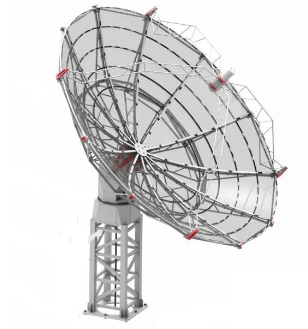
\includegraphics[height = 8cm ]{Figuras/seccion_1/antena_MIA.png}
	\caption{Antena en proceso de construcción para interferómetro MIA}
	\label{fig:antena_mia}
\end{figure}

Este posicionador pertenece a dos proyectos principales y estratégicos dentro de la institución. 
En el caso del interferómetro, se trata de una nueva tecnología hasta ahora inexistente en el observatorio y permitiría incrementar la capacidad científica, tecnológica y observacional del Instituto; mientras que la estación terrena, permitirá establecer enlaces de comunicación con pequeños satélites como parte de las actividades del IAR en el segmento aeroespacial.
%El caso del interferometro, permite mejorar la recepción de las antenas principales de la institución. En el caso de la estación terrena, permite vender el servicio a terceros, y esto permite un ingreso constante al organismo. 

Actualmente el posicionador que se ha desarrollado se encuentra instalado pero tiene la limitación de funcionar con un solo programa (Gpredict), y no puede realizar el seguimiento de radiofuentes. A Este software debe agregar estas radiofuentes, o adicionarle la comunicación con otro software de seguimiento.  

Se desea mejorar incluyendo independencia de software, o mecanismos de manejo remoto, mediante protocolos existentes para las antenas principales. En la figura \ref{fig:antenas_main} se muestran las dos antenas principales del organismo. 

%% 
El sistema de apuntamiento, debe realizar el seguimiento automático (de posición astronómica) de los puntos del cielo, ya sean satélites o radiofuentes. En el caso de no realizar seguimientos, debe permanecer en la posición denominada cenit.En este caso, el sistema debe ser a lazo cerrado todo el tiempo, siguiendo una referencia, que viene dada por una computadora/software, dentro de ciertos margenes. 
Adicionalmente, al estar en un lugar remoto, dentro del organismo, debe poseer telemetria, ya que pueden existir condiciones climaticas adversas en las cuales la antena no podría operarse (ejemplo, viento, granizo, ya que en estos casos, la antena actúa como una vela de barco). El sistema a realizar tiene el diagrama en bloques mostrado en la figura \ref{fig:bloques_sistema} 
%imagen de la antena % 

\begin{figure}[h]
	\vspace{-0.05cm}
	\centering
	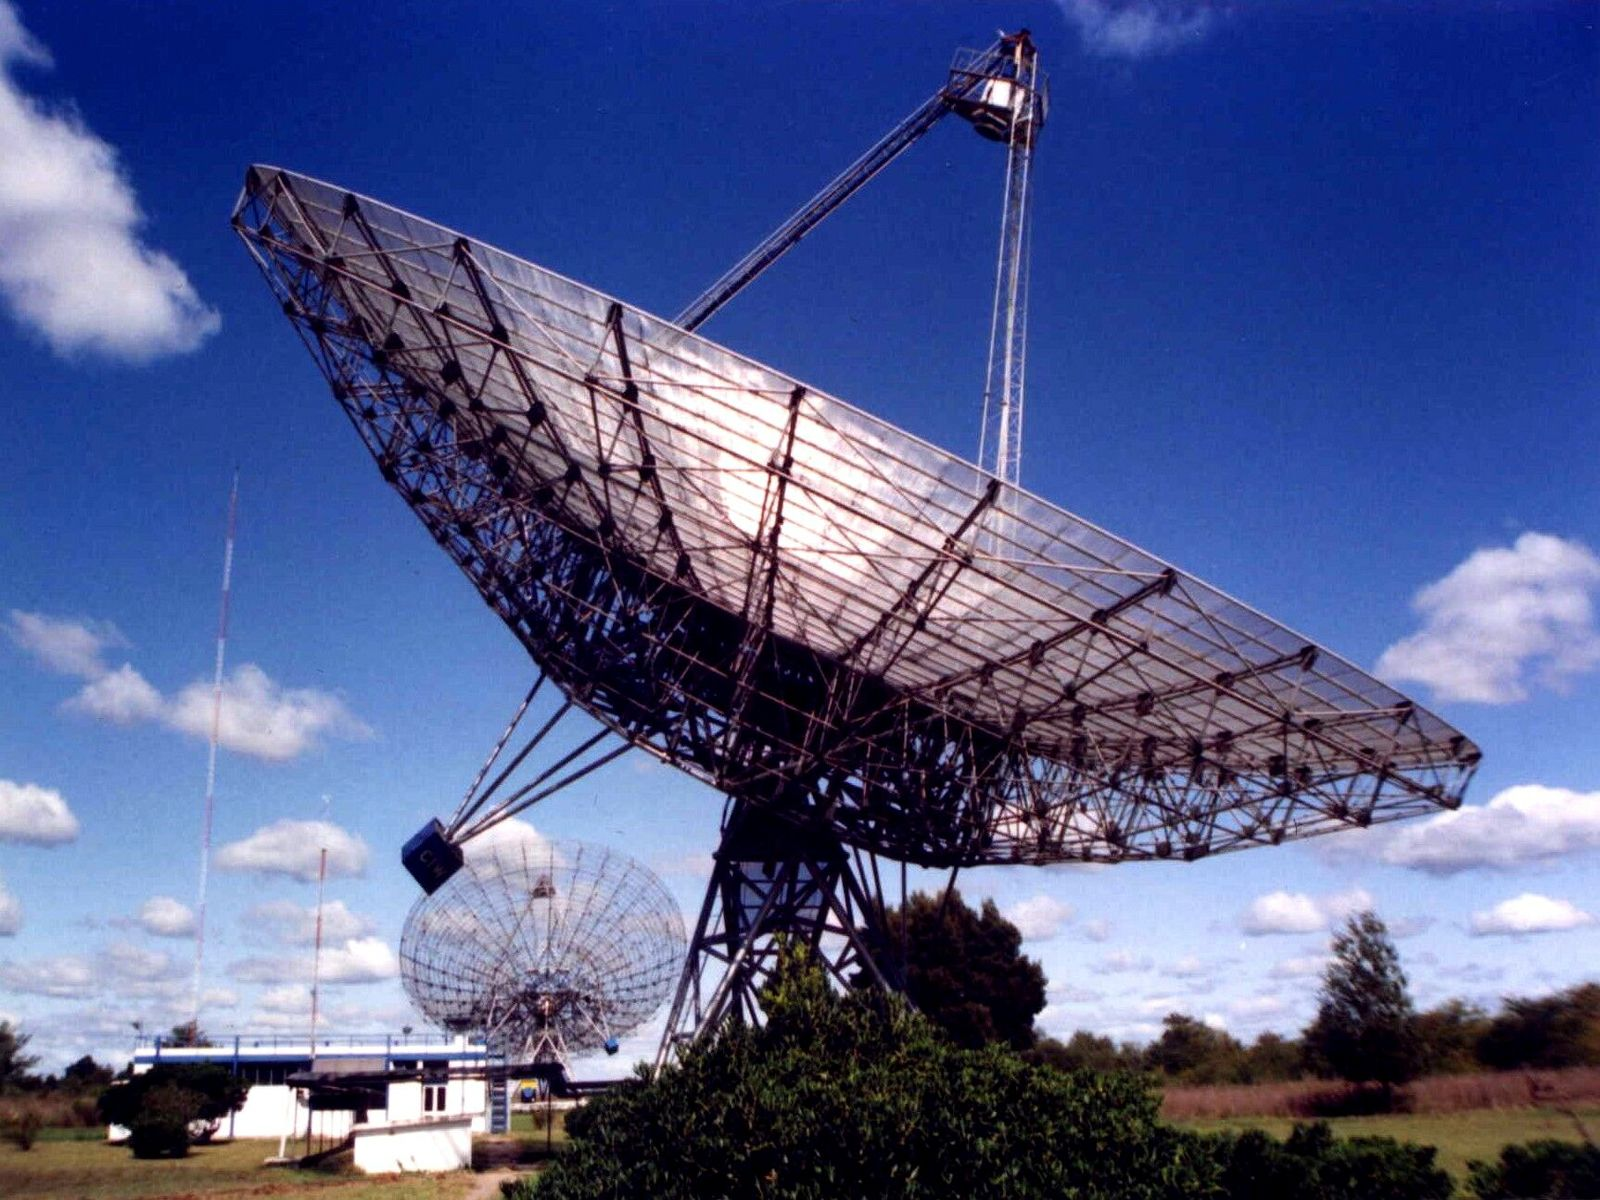
\includegraphics[scale = 0.2]{Figuras/seccion_1/antena_main.jpg}
	\caption{Antenas principales del IAR}
	\label{fig:antenas_main}
\end{figure}

\begin{figure}[h!]
	\vspace{-0.1cm}
	\centering 
	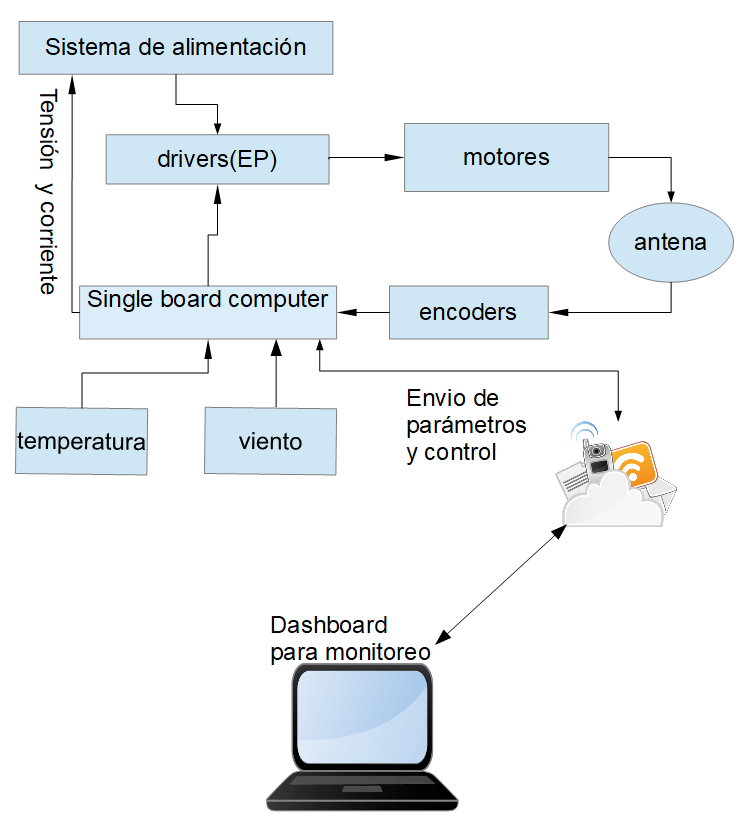
\includegraphics[height=12cm,width =\textwidth]{Figuras/seccion_1/interferometria.png}
	\caption{Diagrama en bloques del sistema }
	\label{fig:bloques_sistema}
\end{figure} 



\section{2. Identificación y análisis de los interesados}
\label{sec:interesados}

\begin{table}[ht]
%\caption{Identificación de los interesados}
%\label{tab:interesados}
\renewcommand {\arrayrulewidth}{1pt}
\begin{tabularx}{\linewidth}{@{}|l|X|X|l|@{}}
	\hline
	\rowcolor[HTML]{C0C0C0} 
	Rol           & Nombre y Apellido & Organización 	& Puesto 	\\ \hline
	Auspiciante   & -                 &  -             	& -        	\\ \hline
	Cliente       & -  			      &	 -				& -       	\\ \hline
	Impulsor      &  -                & -             	& -       	\\ \hline
	Responsable   & \authorname       & IAR        	    & Ing desarrollo firmware/hardware 	\\ \hline
	Colaboradores & Martín Salibe     & IAR             & Responsable de transferencia \\
				  &  Guillermo Gancio & IAR             & Responsable de observatorio \\ \hline
	Orientador    & \supname	      & \pertesupname 	& Director Trabajo final \\ \hline
	Equipo        & Eliseo Diaz \newline 
	Matias Contreras          & IAR              	& Responsables de fabricación de PCB y 3D  	\\ \hline
	Opositores    &  -                 & -             	& -        	\\ \hline
	Usuario final & Facundo Aquino     & IAR           	& Operador de antena  y diseñador PCB    	\\ \hline
\end{tabularx}
\end{table}




\section{3. Propósito del proyecto}
\label{sec:proposito}
	El propósito de este proyecto es realizar un sistema de apuntamiento para una antena (ver figura \ref{fig:antena_mia}),esta antena, debe ponerse en el cenit, en caso de no realizarse ningún tipo de seguimiento, ya que este punto, es el punto de equilibrio mecánico. Una vez finalizado este desarrollo, se va a  replicar en otras tres antenas de iguales características. 


\section{4. Alcance del proyecto}
\label{sec:alcance}
El proyecto incluye los siguientes alcances 

\begin{itemize}
	\item Desarrollo de firmware/software/hardware para realizar el movimiento de los motores de posición 
	\item  Documentación de software/firmware/hardware por separado
	\item  Desarrollo del protocolo de comunicación entre encoders y PC
	\item  Integración del producto con el sistema mecánico de movimiento
	\item Planes de testing para software y hardware. 
	
\end{itemize}

El proyecto, no contempla aspectos relacionados a la seguridad de la información, y selección de los motores para el posicionamiento.  


\section{5. Supuestos del proyecto}
\label{sec:supuestos}
	Para el desarrollo, se supone que se tiene acceso a los siguientes items : 
	\begin{itemize}
		\item Máquina con sistema operativo linux o similar. 
		\item Los recursos de hardware y software se proveen por la institución, así como su documentación
		\item Se tiene acceso a los desarrollos previos realizados para el control de la antena. 
		\item El sistema mecánico se debe armar antes de octubre/noviembre 2022, que esta a cargo del departamento de mecánica. En caso de no realizarse, se verá la forma de simular en algún tipo de software
%		\item 
		\item El proyecto esta inmerso dentro de un plan estratégico dentro de la institución
		\item Los componentes se encuentran en el mercado local, y en el caso de importarse, se realizará con la suficiente antelación. 
		\item La estructura mecánica de movimiento de la antena, estará lista antes de la finalización del presente proyecto. 

	\end{itemize}

\section{6. Requerimientos}
\label{sec:requerimientos}

\begin{enumerate}
	\item Requerimientos funcionales
		\begin{enumerate}
			\item Debe tener un sistema de control de posición
			\item Debe poseer un Webserver embebido para monitoreo de variables ambientales y indicar su estado de operación (tracking, untracking, zenit, y calibrate). 
			\item Debe implementarse lecturas de posicionamiento, lecturas de viento, temperatura y potencia consumida por el mismo. 
			\item Debe conectarse a red local LAN, mediante cable ethernet RJ45 
			\item  Cortar el uso cuando el viento supere la velocidad máxima de operación mecánica de la antena, y volverla a su posición de equilibrio en el zenit 
			\item Debe tener un sistema de calibración a demanda por el operario de la antena 
			\item Realizar de un software central con capacidad de manejar los periféricos del single board computer, y lectura de viento, tensión, corriente, y posición angular de la antena
			\item Realizar un software que se pueda conectar con los programas Gpredict, Stelarium y el existente en el IAR para el manejo de las antenas principales. 
			\item En caso de adicionar otro programa distinto(Gpredict, stellarium o ya existente en el IAR) se debe actualizar el software del sistema posicionador. 
			\item Solo puede realizar una operación de seguimiento. En caso de estar realizando el seguimiento de algún satelite/radiofuente, se le debe informar de dicha operación, y el operario tendrá que esperar que se termine la operación actual  
		\end{enumerate}
	\item Requerimientos de documentación
		\begin{enumerate}
			\item Debe seguir la numeración y formato de los documentos establecidos por el IAR. 
			\item Documentación sobre protocolos de comunicación via ethernet y de los programas involucrados, y trama de mensajes 
			\item Manual de operación de la antena para operarios 
			\item Manual de operación para actualización de software 
			\item Documentación de software y hardware. 
			\item Manual de procedimientos de testing de software y hardware	
	\end{enumerate}
	\item Requerimientos de interfaces
		\begin{enumerate}
			\item Los encoders estarán alineados con los dos ejes principales de movimiento de la antena 
			\item Deberá utilizarse una red electrica para conectar el posicionador
		\end{enumerate}
	\item Requerimiento de testing
		\begin{enumerate}
			\item Medir señal de control de posición de los motores
			\item Webserver embebido, testing de señales sobre la placa con osciloscopio
			\item Realizar el seguimiento de una radiofuente, e intentar realizar más de una conexión simultanea. 
			\item Ver la señal de control mínima a partir de la cual los motores son capaces de mover la antena. 
			\item Realizar experiencia de rebote lunar con stellarium (esto ya se ha realizado con anterioridad con las antenas principales de la institución). El objetivo es corroborar la calibración del mismo y la comunicación con el software  

		\end{enumerate}
\end{enumerate}

\section{7. Historias de usuarios (\textit{Product backlog})}
\label{sec:backlog}

\begin{consigna}{red}
Descripción: En esta sección se deben incluir las historias de usuarios y su ponderación (\textit{history points}). Recordar que las historias de usuarios son descripciones cortas y simples de una característica contada desde la perspectiva de la persona que desea la nueva capacidad, generalmente un usuario o cliente del sistema. La ponderación es un número entero que representa el tamaño de la historia comparada con otras historias de similar tipo.

El formato propuesto es: "como [rol] quiero [tal cosa] para [tal otra cosa]."

Se debe indicar explícitamente el criterio para calcular los \textit{story points} de cada historia
\end{consigna}

\section{8. Entregables principales del proyecto}
\label{sec:entregables}

\begin{consigna}{red}

Los entregables del proyecto son (ejemplo):

\begin{itemize}
	\item Manual de uso
	\item Diagrama de circuitos esquemáticos
	\item Código fuente del firmware
	\item Diagrama de instalación
	\item Informe final
	\item etc...
\end{itemize}

\end{consigna}

\section{9. Desglose del trabajo en tareas}
\label{sec:wbs}

\begin{consigna}{red}
El WBS debe tener relación directa o indirecta con los requerimientos.  Son todas las actividades que se harán en el proyecto para dar cumplimiento a los requerimientos. Se recomienda mostrar el WBS mediante una lista indexada:

\begin{enumerate}
\item Grupo de tareas 1
	\begin{enumerate}
	\item Tarea 1 (tantas hs)
	\item Tarea 2 (tantas hs)
	\item Tarea 3 (tantas hs)
	\end{enumerate}
\item Grupo de tareas 2
	\begin{enumerate}
	\item Tarea 1 (tantas hs)
	\item Tarea 2 (tantas hs)
	\item Tarea 3 (tantas hs)
	\end{enumerate}
\item Grupo de tareas 3
	\begin{enumerate}
	\item Tarea 1 (tantas hs)
	\item Tarea 2 (tantas hs)
	\item Tarea 3 (tantas hs)
	\item Tarea 4 (tantas hs)
	\item Tarea 5 (tantas hs)
	\end{enumerate}
\end{enumerate}

Cantidad total de horas: (tantas hs)

Se recomienda que no haya ninguna tarea que lleve más de 40 hs. 

\end{consigna}

\section{10. Diagrama de Activity On Node}
\label{sec:AoN}

\begin{consigna}{red}
Armar el AoN a partir del WBS definido en la etapa anterior. 

%La figura \ref{fig:AoN} fue elaborada con el paquete latex tikz y pueden consultar la siguiente referencia \textit{online}:

%\url{https://www.overleaf.com/learn/latex/LaTeX_Graphics_using_TikZ:_A_Tutorial_for_Beginners_(Part_3)\%E2\%80\%94Creating_Flowcharts}

\end{consigna}

\begin{figure}[htpb]
\centering 
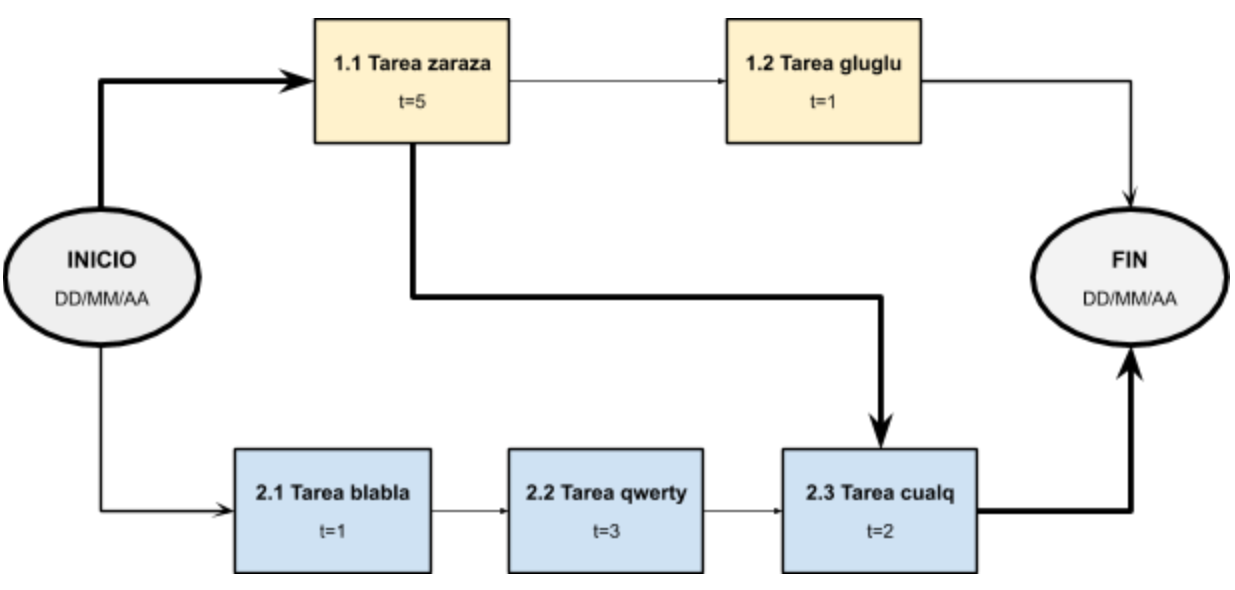
\includegraphics[width=.8\textwidth]{./Figuras/AoN.png}
\caption{Diagrama en \textit{Activity on Node}}
\label{fig:AoN}
\end{figure}

Indicar claramente en qué unidades están expresados los tiempos.
De ser necesario indicar los caminos semicríticos y analizar sus tiempos mediante un cuadro.
Es recomendable usar colores y un cuadro indicativo describiendo qué representa cada color, como se muestra en el siguiente ejemplo:



\section{11. Diagrama de Gantt}
\label{sec:gantt}

\begin{consigna}{red}

Existen muchos programas y recursos \textit{online} para hacer diagramas de gantt, entre los cuales destacamos:

\begin{itemize}
\item Planner
\item GanttProject
\item Trello + \textit{plugins}. En el siguiente link hay un tutorial oficial: \\ \url{https://blog.trello.com/es/diagrama-de-gantt-de-un-proyecto}
\item Creately, herramienta online colaborativa. \\\url{https://creately.com/diagram/example/ieb3p3ml/LaTeX}
\item Se puede hacer en latex con el paquete \textit{pgfgantt}\\ \url{http://ctan.dcc.uchile.cl/graphics/pgf/contrib/pgfgantt/pgfgantt.pdf}
\end{itemize}

Pegar acá una captura de pantalla del diagrama de Gantt, cuidando que la letra sea suficientemente grande como para ser legible. 
Si el diagrama queda demasiado ancho, se puede pegar primero la ``tabla'' del Gantt y luego pegar la parte del diagrama de barras del diagrama de Gantt.

Configurar el software para que en la parte de la tabla muestre los códigos del EDT (WBS).\\
Configurar el software para que al lado de cada barra muestre el nombre de cada tarea.\\
Revisar que la fecha de finalización coincida con lo indicado en el Acta Constitutiva.

En la figura \ref{fig:gantt}, se muestra un ejemplo de diagrama de gantt realizado con el paquete de \textit{pgfgantt}. En la plantilla pueden ver el código que lo genera y usarlo de base para construir el propio.

\begin{figure}[htbp]
\begin{center}
\begin{ganttchart}{1}{12}
  \gantttitle{2020}{12} \\
  \gantttitlelist{1,...,12}{1} \\
  \ganttgroup{Group 1}{1}{7} \\
  \ganttbar{Task 1}{1}{2} \\
  \ganttlinkedbar{Task 2}{3}{7} \ganttnewline
  \ganttmilestone{Milestone o hito}{7} \ganttnewline
  \ganttbar{Final Task}{8}{12}
  \ganttlink{elem2}{elem3}
  \ganttlink{elem3}{elem4}
\end{ganttchart}
\end{center}
\caption{Diagrama de gantt de ejemplo}
\label{fig:gantt}
\end{figure}


\begin{landscape}
\begin{figure}[htpb]
\centering 
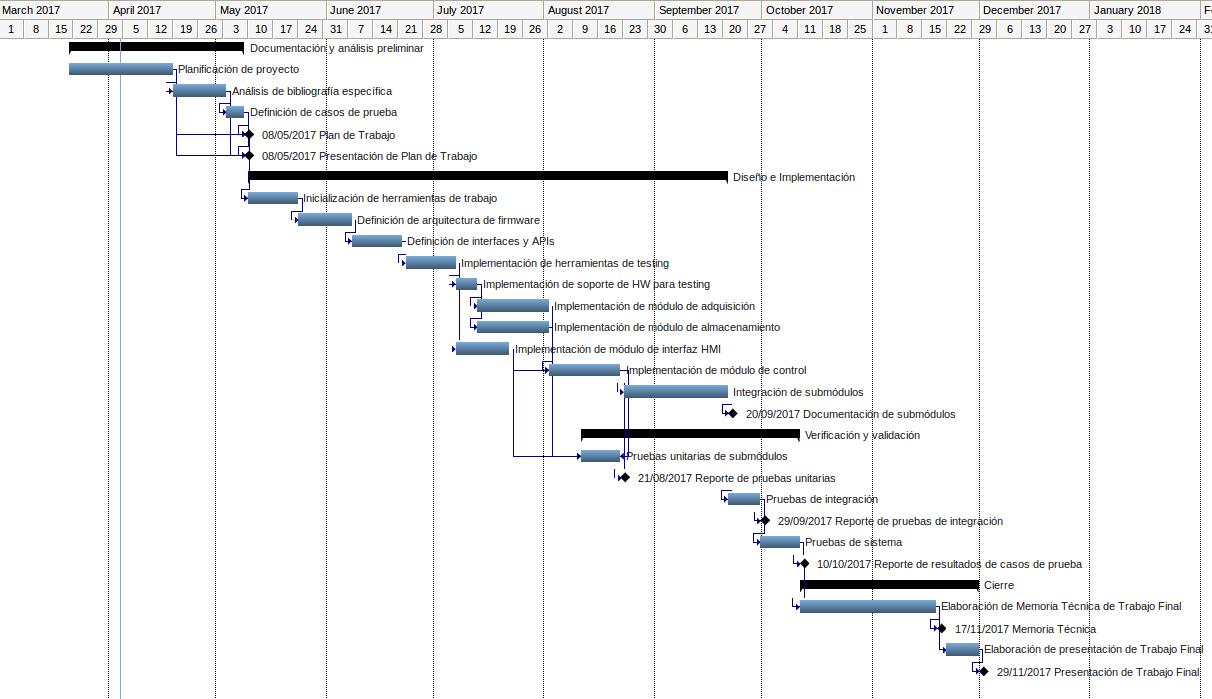
\includegraphics[height=.85\textheight]{./Figuras/Gantt-2.png}
\caption{Ejemplo de diagrama de Gantt rotado}
\label{fig:diagGantt}
\end{figure}

\end{landscape}

\end{consigna}


\section{12. Presupuesto detallado del proyecto}
\label{sec:presupuesto}

\begin{consigna}{red}
Si el proyecto es complejo entonces separarlo en partes:
\begin{itemize}
	\item Un total global, indicando el subtotal acumulado por cada una de las áreas.
	\item El desglose detallado del subtotal de cada una de las áreas.
\end{itemize}

IMPORTANTE: No olvidarse de considerar los COSTOS INDIRECTOS.

\end{consigna}

\begin{table}[htpb]
\centering
\begin{tabularx}{\linewidth}{@{}|X|c|r|r|@{}}
\hline
\rowcolor[HTML]{C0C0C0} 
\multicolumn{4}{|c|}{\cellcolor[HTML]{C0C0C0}COSTOS DIRECTOS} \\ \hline
\rowcolor[HTML]{C0C0C0} 
Descripción &
  \multicolumn{1}{c|}{\cellcolor[HTML]{C0C0C0}Cantidad} &
  \multicolumn{1}{c|}{\cellcolor[HTML]{C0C0C0}Valor unitario} &
  \multicolumn{1}{c|}{\cellcolor[HTML]{C0C0C0}Valor total} \\ \hline
 &
  \multicolumn{1}{c|}{} &
  \multicolumn{1}{c|}{} &
  \multicolumn{1}{c|}{} \\ \hline
 &
  \multicolumn{1}{c|}{} &
  \multicolumn{1}{c|}{} &
  \multicolumn{1}{c|}{} \\ \hline
\multicolumn{1}{|l|}{} &
   &
   &
   \\ \hline
\multicolumn{1}{|l|}{} &
   &
   &
   \\ \hline
\multicolumn{3}{|c|}{SUBTOTAL} &
  \multicolumn{1}{c|}{} \\ \hline
\rowcolor[HTML]{C0C0C0} 
\multicolumn{4}{|c|}{\cellcolor[HTML]{C0C0C0}COSTOS INDIRECTOS} \\ \hline
\rowcolor[HTML]{C0C0C0} 
Descripción &
  \multicolumn{1}{c|}{\cellcolor[HTML]{C0C0C0}Cantidad} &
  \multicolumn{1}{c|}{\cellcolor[HTML]{C0C0C0}Valor unitario} &
  \multicolumn{1}{c|}{\cellcolor[HTML]{C0C0C0}Valor total} \\ \hline
\multicolumn{1}{|l|}{} &
   &
   &
   \\ \hline
\multicolumn{1}{|l|}{} &
   &
   &
   \\ \hline
\multicolumn{1}{|l|}{} &
   &
   &
   \\ \hline
\multicolumn{3}{|c|}{SUBTOTAL} &
  \multicolumn{1}{c|}{} \\ \hline
\rowcolor[HTML]{C0C0C0}
\multicolumn{3}{|c|}{TOTAL} &
   \\ \hline
\end{tabularx}%
\end{table}


\section{13. Gestión de riesgos}
\label{sec:riesgos}

\begin{consigna}{red}
a) Identificación de los riesgos (al menos cinco) y estimación de sus consecuencias:
 
Riesgo 1: detallar el riesgo (riesgo es algo que si ocurre altera los planes previstos de forma negativa)
\begin{itemize}
	\item Severidad (S): mientras más severo, más alto es el número (usar números del 1 al 10).\\
	Justificar el motivo por el cual se asigna determinado número de severidad (S).
	\item Probabilidad de ocurrencia (O): mientras más probable, más alto es el número (usar del 1 al 10).\\
	Justificar el motivo por el cual se asigna determinado número de (O). 
\end{itemize}   

Riesgo 2:
\begin{itemize}
	\item Severidad (S): 
	\item Ocurrencia (O):
\end{itemize}

Riesgo 3:
\begin{itemize}
	\item Severidad (S): 
	\item Ocurrencia (O):
\end{itemize}


b) Tabla de gestión de riesgos:      (El RPN se calcula como RPN=SxO)

\begin{table}[htpb]
\centering
\begin{tabularx}{\linewidth}{@{}|X|c|c|c|c|c|c|@{}}
\hline
\rowcolor[HTML]{C0C0C0} 
Riesgo & S & O & RPN & S* & O* & RPN* \\ \hline
       &   &   &     &    &    &      \\ \hline
       &   &   &     &    &    &      \\ \hline
       &   &   &     &    &    &      \\ \hline
       &   &   &     &    &    &      \\ \hline
       &   &   &     &    &    &      \\ \hline
\end{tabularx}%
\end{table}

Criterio adoptado: 
Se tomarán medidas de mitigación en los riesgos cuyos números de RPN sean mayores a...

Nota: los valores marcados con (*) en la tabla corresponden luego de haber aplicado la mitigación.

c) Plan de mitigación de los riesgos que originalmente excedían el RPN máximo establecido:
 
Riesgo 1: plan de mitigación (si por el RPN fuera necesario elaborar un plan de mitigación).
  Nueva asignación de S y O, con su respectiva justificación:
  - Severidad (S): mientras más severo, más alto es el número (usar números del 1 al 10).
          Justificar el motivo por el cual se asigna determinado número de severidad (S).
  - Probabilidad de ocurrencia (O): mientras más probable, más alto es el número (usar del 1 al 10).
          Justificar el motivo por el cual se asigna determinado número de (O).

Riesgo 2: plan de mitigación (si por el RPN fuera necesario elaborar un plan de mitigación).
 
Riesgo 3: plan de mitigación (si por el RPN fuera necesario elaborar un plan de mitigación).

\end{consigna}


\section{14. Gestión de la calidad}
\label{sec:calidad}

\begin{consigna}{red}
Para cada uno de los requerimientos del proyecto indique:
\begin{itemize} 
\item Req \#1: copiar acá el requerimiento.

\begin{itemize}
	\item Verificación para confirmar si se cumplió con lo requerido antes de mostrar el sistema al cliente. Detallar 
	\item Validación con el cliente para confirmar que está de acuerdo en que se cumplió con lo requerido. Detallar  
\end{itemize}

\end{itemize}

Tener en cuenta que en este contexto se pueden mencionar simulaciones, cálculos, revisión de hojas de datos, consulta con expertos, mediciones, etc.  Las acciones de verificación suelen considerar al entregable como ``caja blanca'', es decir se conoce en profundidad su funcionamiento interno.  En cambio, las acciones de validación suelen considerar al entregable como ``caja negra'', es decir, que no se conocen los detalles de su funcionamiento interno.

\end{consigna}

\section{15. Procesos de cierre}    
\label{sec:cierre}

\begin{consigna}{red}
Establecer las pautas de trabajo para realizar una reunión final de evaluación del proyecto, tal que contemple las siguientes actividades:

\begin{itemize}
	\item Pautas de trabajo que se seguirán para analizar si se respetó el Plan de Proyecto original:
	 - Indicar quién se ocupará de hacer esto y cuál será el procedimiento a aplicar. 
	\item Identificación de las técnicas y procedimientos útiles e inútiles que se emplearon, y los problemas que surgieron y cómo se solucionaron:
	 - Indicar quién se ocupará de hacer esto y cuál será el procedimiento para dejar registro.
	\item Indicar quién organizará el acto de agradecimiento a todos los interesados, y en especial al equipo de trabajo y colaboradores:
	  - Indicar esto y quién financiará los gastos correspondientes.
\end{itemize}

\end{consigna}


\end{document}
